\section{Wstęp}
\suppressfloats[t]  %żeby obiekt ruchomy (rysunek, tablica, itp.) nie pojawił się u góry tej strony
\subsection{Cel i~zakres pracy}
Sprawdzenie możliwosci wykorzystania internetu rzeczy oraz bezzałogowych statków powietrznych przy wspomaganiu prowadzenia akcji ratowniczej. Fizyczne zaprojektowanie i wykonanie kompletnego systemu, cześci działającej na pokładzie statku powietrznym, oraz części diałającej na ziemi. Przetestowanie systemu w warunkach symulowanej akcji ratunkowej. Potwierdzenie lub zaprzeczenie użytecznosci projektowanego systemu, wykazanie wad i zalet systemu.
\subsection{Tło projektu}
Pomysł projektu nasunęli organizatorzy konferencji "Parada Robotów 2017" i zarazem konkursu "Droniada" \cite{droniada}. Zadaniem uczestników konkursu było wspomaganie ewakuacji medycznej 10 osób po ataku huraganowego wiatru, przy użyciu bezzałogowców w locie autonomicznym, lub ewentualnie półautonomicznym, oraz tzw. beaconów. W tym dokumencie opiszę system lokkalizowania poszkodowanych osób, który stworzony został na potrzeby wspomnianego wyżej konkursu.

\begin{figure}[!th]
    \centering
    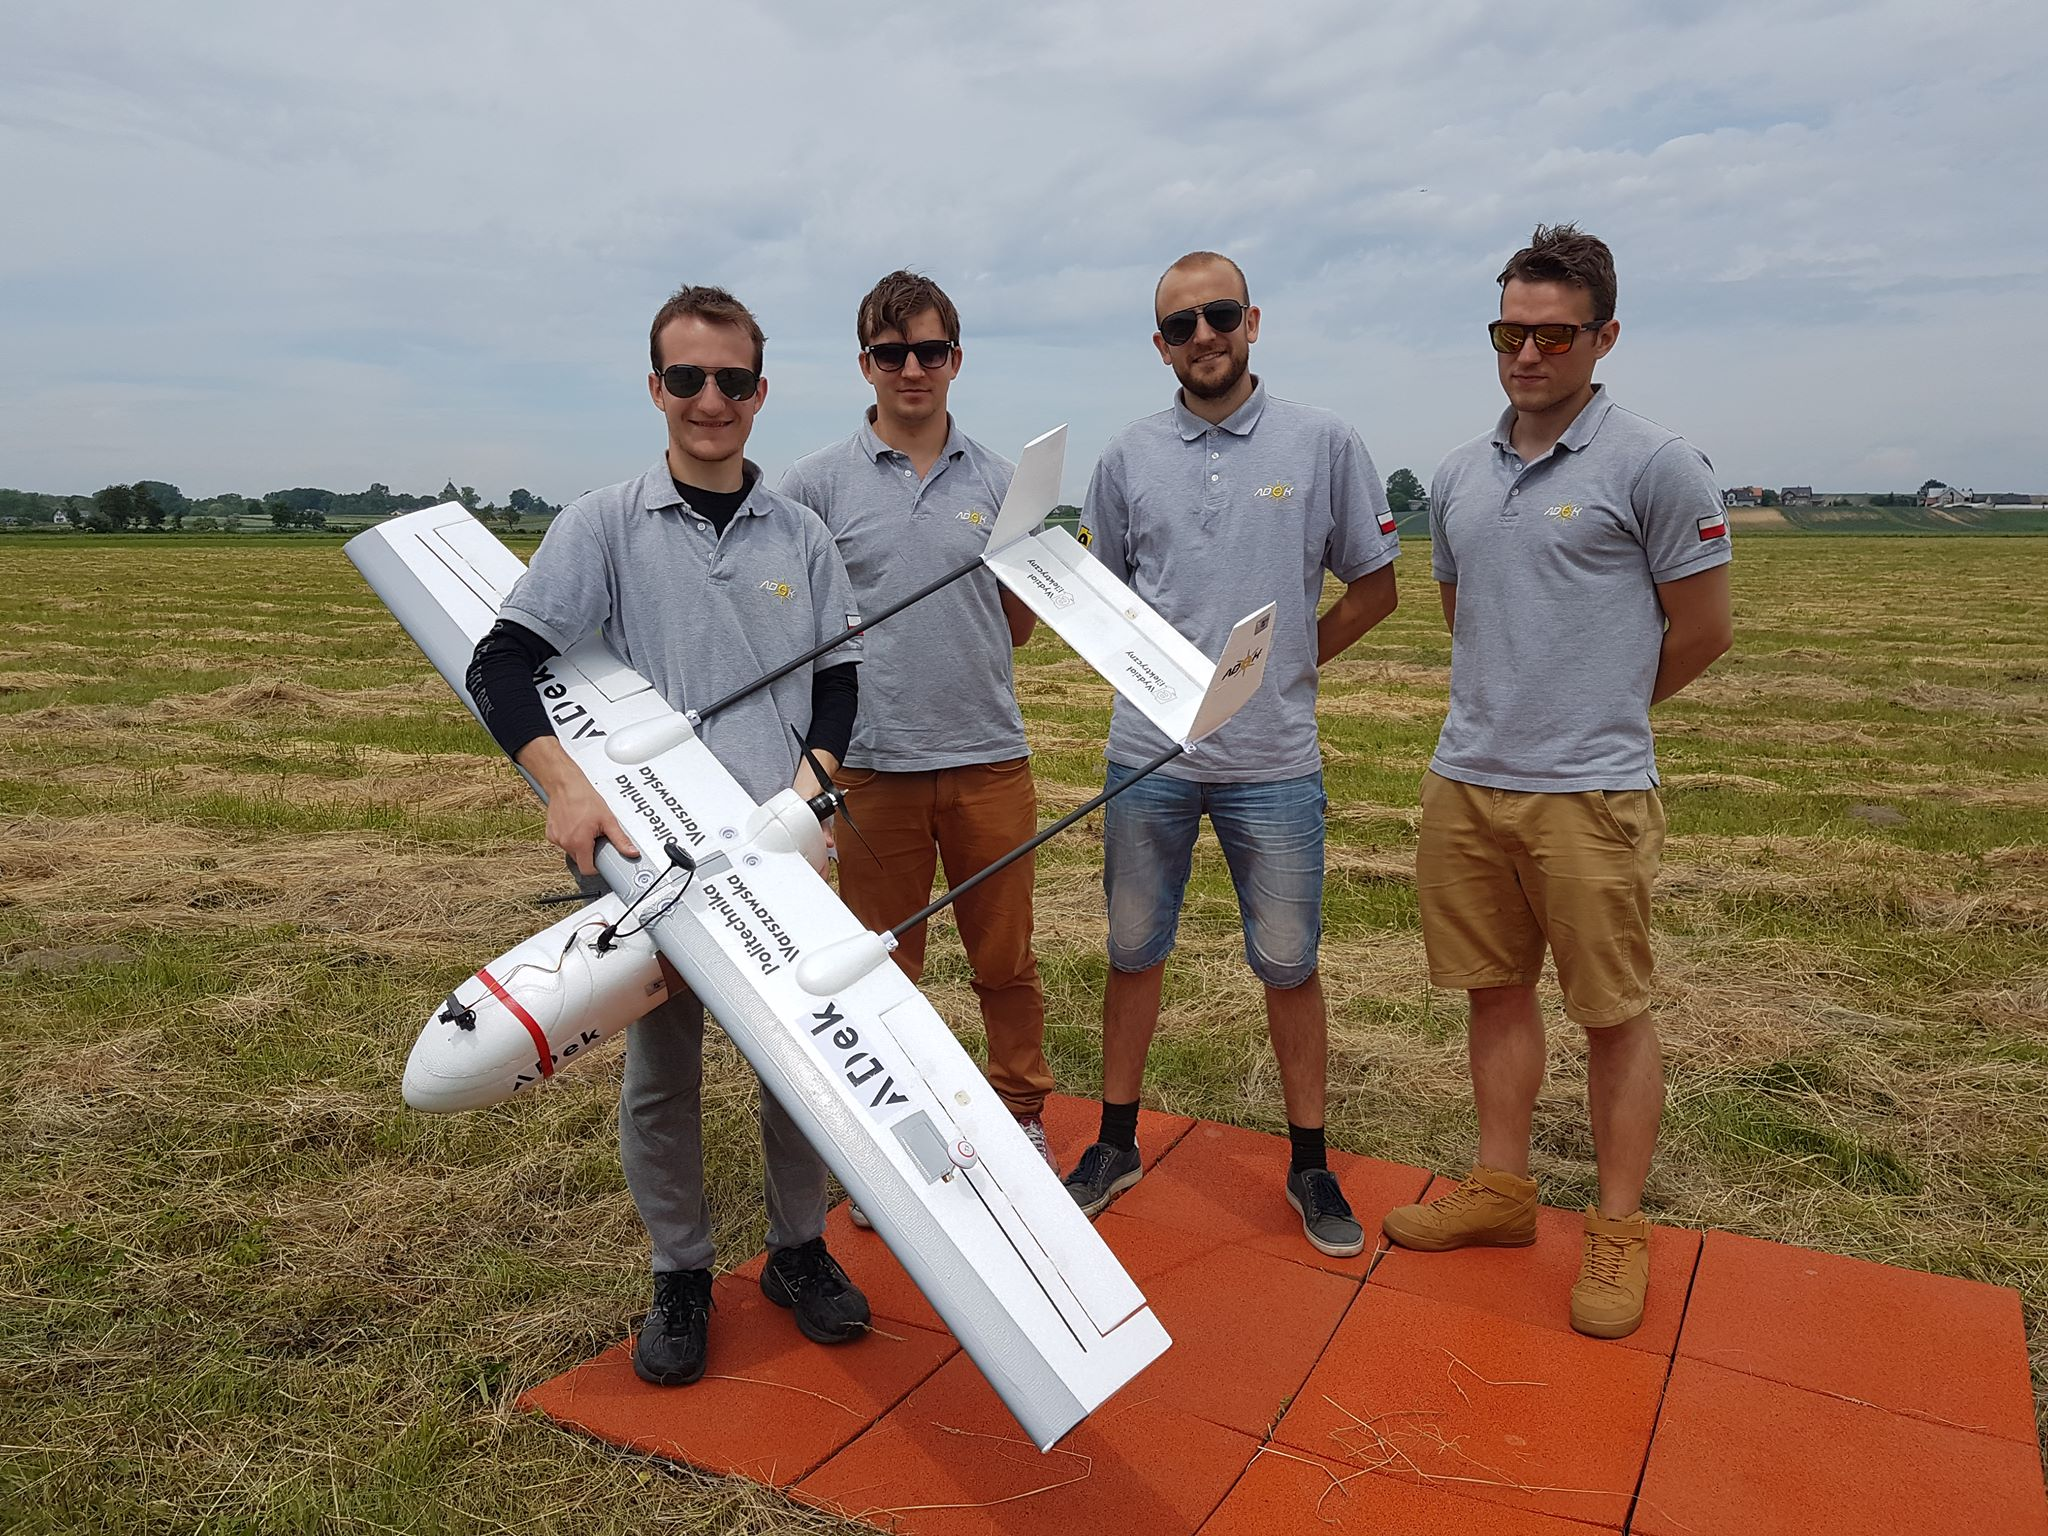
\includegraphics[width=15cm]{zalaczniki/obrazy/droniada.jpg}
    \caption{Nasz zespół na konkursie "Droniada".}
    \label{fig:triage}
\end{figure}

\subsection{Wprowadzenie do zagadnienia}
Projektowany system składał się z kliku części. Część pierwsza to poszkodowane w katastrofie osoby, którym ratownicy medyczni przypisują kolejne kolory przy pomocy beaconów, i tak kolor czerwony jest przyporządkowany do osób co do których wymagana jest natychmiastowa ewakuacja, kolorem żółtym oznaczone zostają osoby które wymagają pilnej ewakuacji (mniejszy priorytet), kolorem zielonym osoby które chodzą o własnych siłach, natomiast kolorem czarnym zgony, osoby których ciała zostaną usunięte dopiero po zakończeniu akcji ratowania życia. Jest to tzw. system znaczników Triage \cite{triage}.

\begin{figure}[!th]
    \centering
    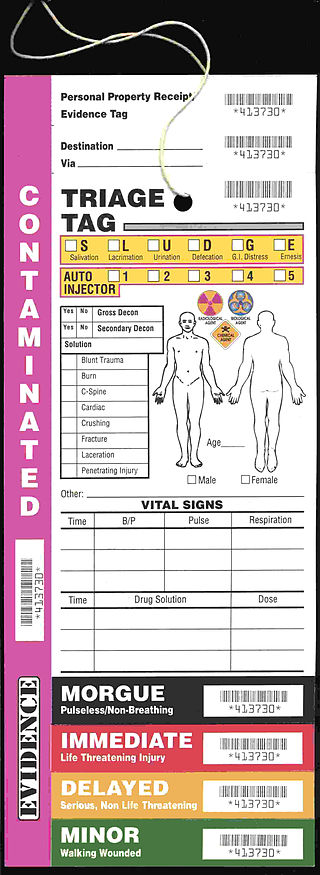
\includegraphics[width=5cm]{zalaczniki/obrazy/triage_tag.jpg}
    \caption{Typowy znacznik systemu Triage, używany w akcjach ratowniczych \cite{triage}.}
    \label{fig:triage}
\end{figure}

Kolejnym komponentem był statek powietrzny który miał za zadanie zbieranie, nadawanych dookólnie przez beacony, sygnałów i umiejscawianie ich na płaszczyźnie mapy. Taki statek musiał zostać wyposażony w odbiornik bluetooth w wersji conajmniej 4.0 i odpowiednie oprogramowanie.

Ostatnim elementem systemu był system naziemny (ang. \textit{Ground Station}). System ten zbierał zlokalizowane przez statek powietrzny sygnały i wyświetlał je na mapie, dodatkowo aproksymując pozycję realną beacona na mapie.

W kolejnych rozdziałach będę przybliżał powyższe komponenty systemu.

\section{Internet rzeczy}
\subsection{Koncepcja pomysłu internetu rzeczy}
Internet rzeczy (ang. \textit{Internet of Things - IoT}) to idea która zakłada że wszystko można podłączyć do sieci internet \cite{iot}, wszystko to znaczy pojazd, budynek, i inne rzeczy wyposażone w elektroniczny system wbudowany z sensorami, aktorami oraz interfejs sieciowy, dzięki czemu możliwa jest wymiana danych. 


\subsection{Sprzęt i BLE}
Głównym komponentem systemu jest tzw. beacon, jest to urządzenie małej mocy które, w z góry określonych interwałach czasowych, nadaje dookólnie ramki danych poprzez bluetooth. Ważne jest że beacon ma zaimplementowany bluetooth w wersji 4.0 (lub wyższej) potocznie nazywany BLE (ang. \textit{Bluetooth Low Energy}).
Z czego składa się IoT, jakich urządzeń używa, czym różni się bluetooth 4.0 od wcześniejszych wersji. Czym charakteryzują się kolejne wersji 4.1, 4.2, 4.3. Co to jest RSSI i jak je wykorzystać do określania pozycji, czy jest dokładne.
\subsection{Komponenty IoT wykorzystane w tworzonym systemie}
Beacony, gateway, urządzenia odbiorcze.

\section{Bezzałogowe statki powietrzne}
\subsection{Czym są UAV}
Bezzałogowy statek powietrzny, dron– statek powietrzny, który nie wymaga do lotu załogi obecnej na pokładzie oraz nie ma możliwości zabierania pasażerów, pilotowany zdalnie lub wykonujący lot autonomicznie...
\subsection{Rola UAV w projektowanym systemie}
Po co UAV, jak będziemy je wykorzystywać, czy nie lepiej skorzystać z czegoś innego.
\subsection{Autonomiczna misja}
Jak zaplanować, czy jest możliwa, jakie są obostrzenia, co mogę, a czego nie mogę zrobić w misji autonomicznej.
\subsection{Bezpieczeństwo stosowania UAV w misji ratunkowej}
Czy nie stanie się tak że trzeba będzie ratować ratownika, na co trzeba uważać, jak trzeba się oznaczyć, o czym należy pamiętać.

\section{Koncepcja techniczna systemu}
\subsection{Architektura tworzonego systemu}
Komponenty systemu, podział odpowiedzialności pomiędzy sprzęt i ludzi, protokoły pomiędzy urządzeniami, fale radiowe, zakłócenia...
\subsection{Schemat blokowy rozwiązania}
\subsection{Algorytm pracy}
Co po kolei się włącza, kto za co odpowiada i w którym momencie należy coś wyzwolić, pod jakimi warunkami, kto to ma zrobić.
\subsection{Podłączenie wielu statków w jeden system}
Czy jest możliwe, czy jest bezpieczne, jak nimi sterować, czy się wzajemnie nie zakłócają
\subsection{Sterowanie autonomiczne}
Jak to robić, jak unikać kolizji, jak plaować misje
\subsection{Bezpieczeństwo użytkowania}
O czym powienien pamiętać ratownik tak żeby sam nie potrzebował pomocy
\subsection{Aspekty mechaniczne systemu}

\section{Problemy i próba ich rozwiązania}
\subsection{Krótki czas lotu UAV}
\subsection{Zawodność linku telemetrycznego}
\subsection{Wrażliwość systemu na sytuacje wyjątkowe}
\subsection{Problemy sprzętowe}

\section{Testy systemu}
Loty autonomiczne, wyznaczanie charakterystyk siły sygnału bluetooth...

\section{Konkurs}
Jak nam poszło, jak dokładnie udało się określić pozycje, problemy podczas konkursu, wypadki, wyjątkowe sytuacje. Jak sprawdził się nasz osprzęt.

\section{Podsumowanie}
\subsection{Wnioski}
\subsection{Plany na przyszłość}
